% Appendix Template

\chapter{Nachverarbeitung} % Main appendix title

\label{AppendixG} % Change X to a consecutive letter; for referencing this appendix elsewhere, use \ref{AppendixX}
\begin{figure}[h]
    \centering
    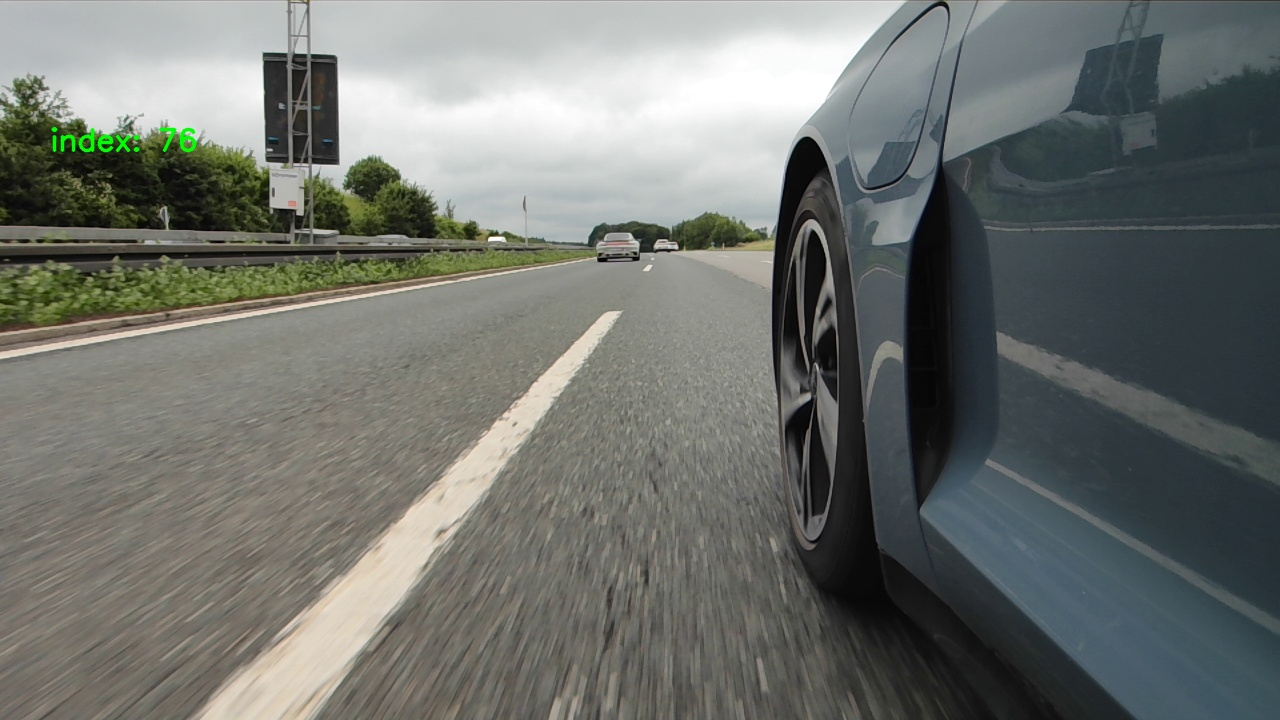
\includegraphics[width=\linewidth]{Figures/M2_T15_F76_left_steps/example.jpg}
    \caption{Messung 2 Trigger 15 Frame 76 links}
    \label{fig:M2_T15_F76_left_example}
\end{figure}
\begin{figure}[h]
    \centering
    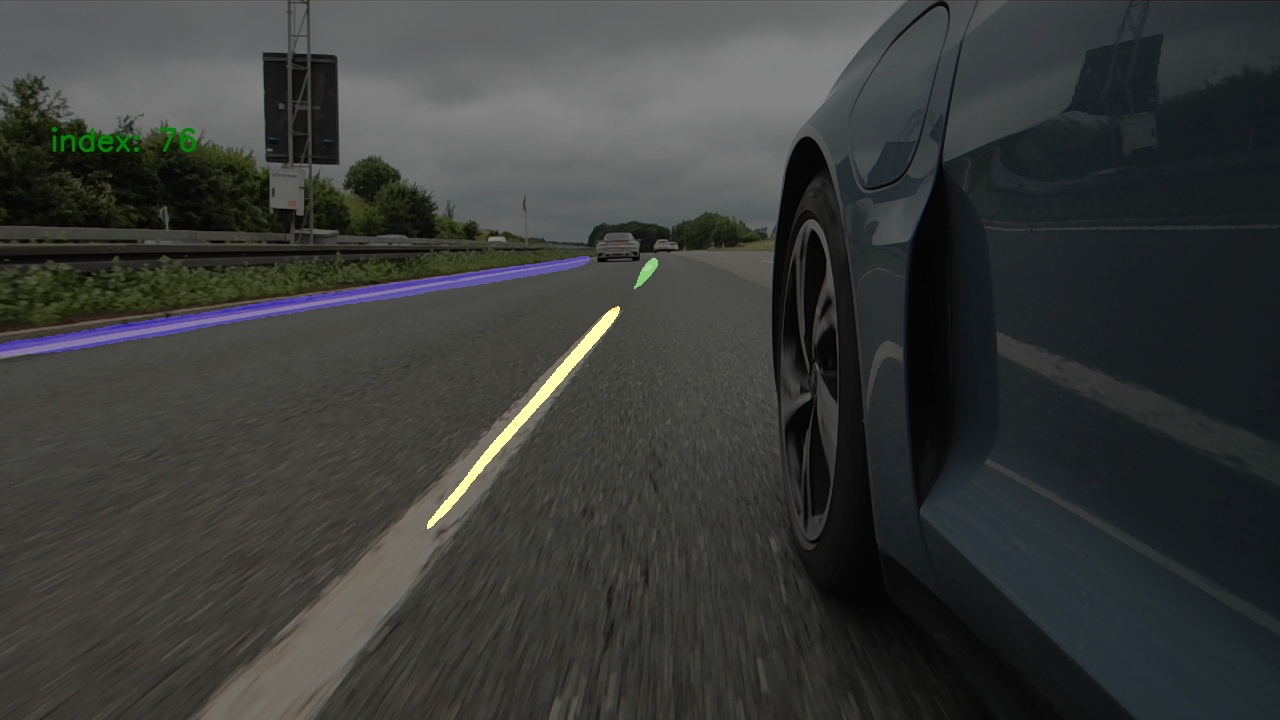
\includegraphics[width=\linewidth]{Figures/M2_T15_F76_left_steps/segments.jpg}
    \caption{Messung 2 Trigger 15 Frame 76 links zusammenhängende Segmente}
    \label{fig:M2_T15_F76_left_segments}
\end{figure}
\begin{figure}[h]
    \centering
    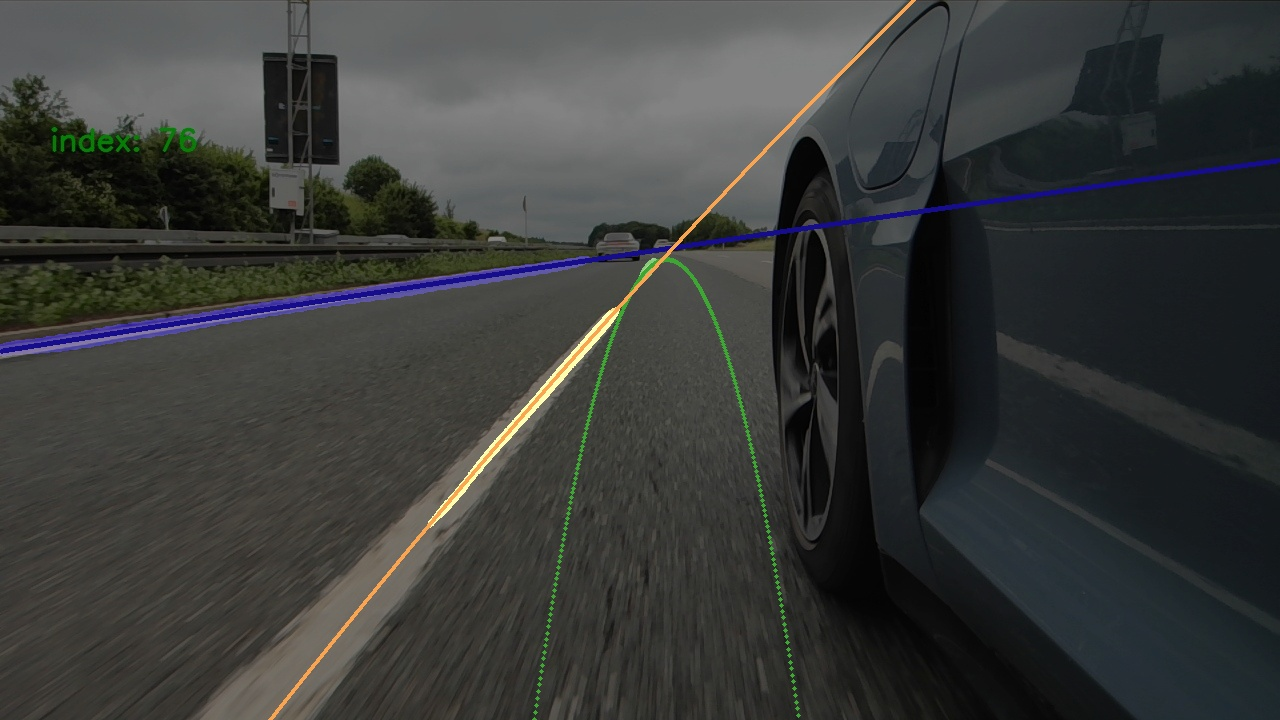
\includegraphics[width=\linewidth]{Figures/M2_T15_F76_left_steps/polys.jpg}
    \caption{Messung 2 Trigger 15 Frame 76 links zusammenhängende Segmente}
    \label{fig:M2_T15_F76_left_polys}
\end{figure}
\begin{figure}[h]
    \centering
    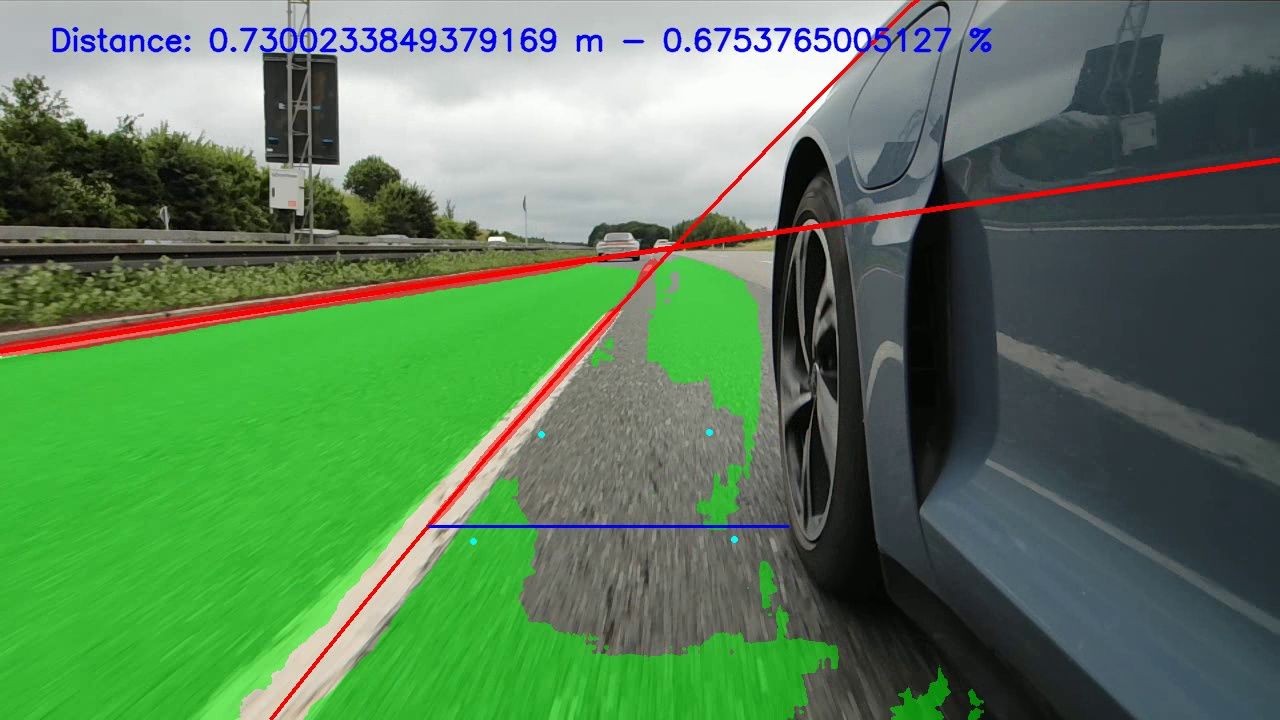
\includegraphics[width=\linewidth]{Figures/M2_T15_F76_left_steps/result.jpg}
    \caption{Messung 2 Trigger 15 Frame 76 links Ergebnis}
    \label{fig:M2_T15_F76_left_result}
\end{figure}
